\section{Deep Learning}\label{sec:deep-learning}

Deep learning method is part of machine learning methods based on artificial neural network with representation learning.
The learning process can be supervised, semi-supervised, or unsupervised.

There is a very large variety of deep learning architectures, some of them are specialized in some fields meanwhile others have a broader usage, especially, there are Convolutional Neural Network and Transformers.

\subsection{Convolutional Neural Network}\label{subsec:conv-neural-network}
The \gls{cnn} is a class of artificial neural network, it is used in almost every imagery related task, such as image classification, object detection, image segmentation, etc.

The CNN take an input image, assign importance (learnable weights and biases) and process the input image by using the convolution operation extracting features.
There are two important parameter in the convolution operation, the kernel size and the stride.
The kernel is a matrix which is used to perform the convolution operation, the stride is the number of pixels the kernel slides over the input image to produce a new pixel.
With stride we can control the size of the output image, if the stride is equal to 1, the output image will have the same size of the input image, if the stride is equal to 2, the output image will have half the size of the input image.
\begin{figure}[H]
    \centering
    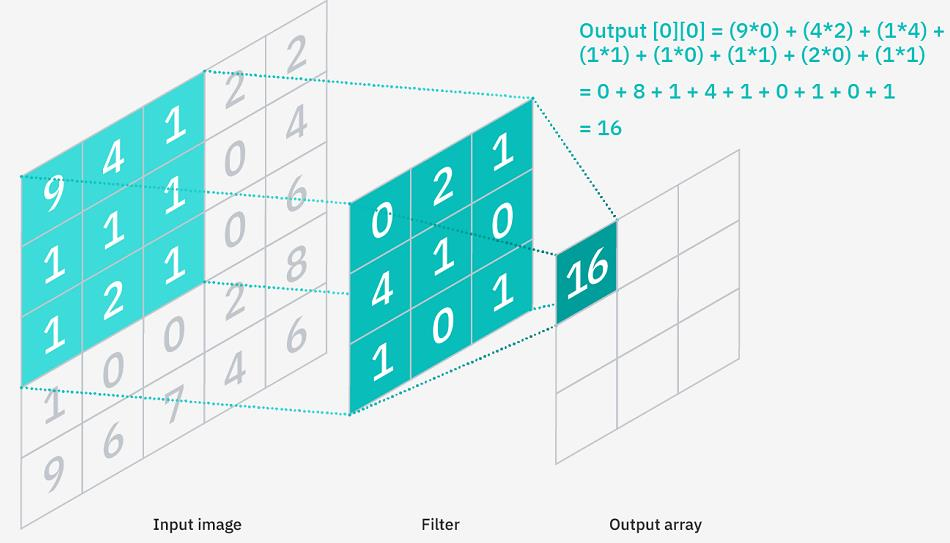
\includegraphics[width=\textwidth]{images/2_convolutions}
    \caption{Convolutions: every single element of the output feature map is obtained by summing the element-wise product between the elements from the input feature map and the kernel. The whole feature map is then obtained sliding the kernel over the input feature map.}
    \label{fig:figure-convolutions}
\end{figure}
More concisely, given the input image $I$ and the kernel $K$, output feature map $O$, the convolution operation is defined as:
\begin{figure}[H]
    \[O_{ij} = \sum_{ij} I_{ij} * K_{ij}\]
    \caption{Convolution operation expression.}
    \label{fig:expression-convolution}
\end{figure}
Increasing the number of layers and combining the pooling layers, the CNN is able to extract more and more complex features, such as edges, lines, shapes, etc.
Then, there are pooling layers, usually max-pooling and average pooling, which can reduce the dimensionality of the feature maps by setting strides \[>=2\], which is useful to reduce the computational cost.
For example, max-pooling is computed as showed in the image:
\begin{figure}[H]
    \centering
    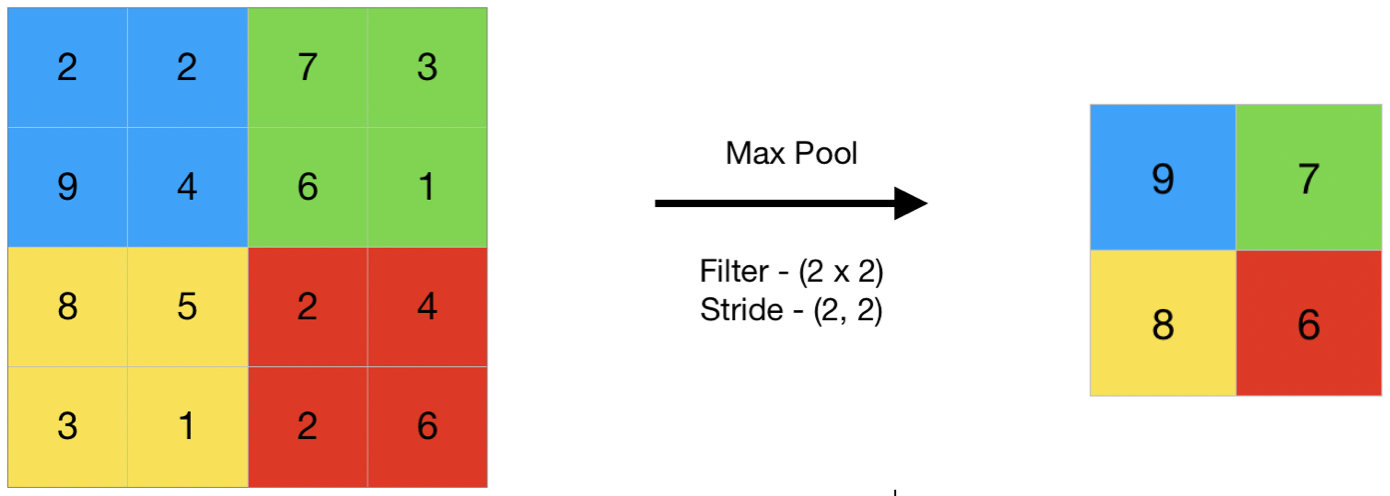
\includegraphics[width=\textwidth]{images/2_max_pooling}
    \caption{Max-pooling: essentially, it strides over the input image and takes the max value of the area covered by the kernel.}
    \label{fig:figure-max-pooling}
\end{figure}
With stride = 2, sliding over the input feature map and taking the maximum value of the window, the dimensionality of the feature map is reduced.
Another important component is the activation function, \gls{relu} is the most used one, it is defined as:
\begin{figure}[H]
    \[ReLU(x) = \max(0, x)\]
    \caption{ReLU activation function.}
    \label{fig:expression-relu}
\end{figure}
Which guarantees the non-linearity of the network, allowing the network to learn more complex features.
These are the main components of a CNN, but there are other components, such as batch normalization and dropout which are used to improve the performance of the network reducing the over-fitting.
\subsection{Transformer}\label{subsec:transformer}
% https://jalammar.github.io/illustrated-transformer/
